%!TEX root = doc.tex
%!TEX output_directory = aux

While there do appear to be a few general and consistent findings in the pruning literature (see the previous section), by far the clearest takeaway is that pruning papers rarely make direct and controlled comparisons to existing methods. This lack of comparisons stems largely from a lack of experimental standardization and the resulting fragmentation in reported results. This fragmentation makes it difficult for even the most committed authors to compare to more than a few existing methods.
% Section~\ref{sec:lessons}
 % Moreover, when such comparisons are made, they often fail to account

% literature suffers from a dearth of meaningful comparisons between methods. This deficiency stems from a lack of experimental standardization, which makes it impractical for new authors to compare to more than a small number of existing methods. % Below, we provide evidence for these claims and highlight pitfalls that should be avoided for future comparisons. % However, as we will discuss in the next section, this is not a result of individual authors making poor choices, but of the field as a whole failing to converge on standard experimental setups.
% In this section, we argue that such a lack of comparisons exists, and that this lack presents a barrier to progress within this field.

% ------------------------------------------------
% \vspace{-1.5mm}
\subsection{Omission of Comparison}
% \vspace{-.25mm}
% ------------------------------------------------

Many papers claim to advance the state of the art, but don't compare to other methods---including many published ones---that make the same claim. % This implies that many such claims are not adequately justified.

% Dozens of papers in our corpus purport to introduce a method that surpasses the current state-of-the-art. A necessary condition for this claim to be true is that the paper outperform any other nominally ``state-of-the-art'' methods existing at the time the paper is written. However, few if any papers in the past decade have been able to demonstrate that they do this. % Indeed, they have not even \textit{compared} to many papers that have a claim to be state-of-the-art.

% ------------------------
% \subsubsection{Ignoring Pre-2010s Methods}
\vspace{-2mm}
\paragraph{Ignoring Pre-2010s Methods}
% ------------------------

% To see this, consider first the fact that t
There was already a rich body of work on neural network pruning by the mid 1990s (see, e.g., Reed's survey \cite{reed_pruning_1993}), which has been almost completely ignored except for Lecun's Optimal Brain Damage \cite{optimal-brain-damage} and Hassibi's Optimal Brain Surgeon \cite{optimal-brain-surgeon}. Indeed, multiple authors have rediscovered existing methods or aspects thereof, with \citet{learning-both} reintroducing the magnitude-based pruning of \citet{janowsky_pruning_1989}, \citet{snip} reintroducing the saliency heuristic of \citet{mozer_skeletonization:_1989}, and \citet{soft-filter-pruning} reintroducing the practice of ``reviving'' previously pruned weights described in \citet{early-brain-damage}.
\begin{figure}[t]
\begin{center}
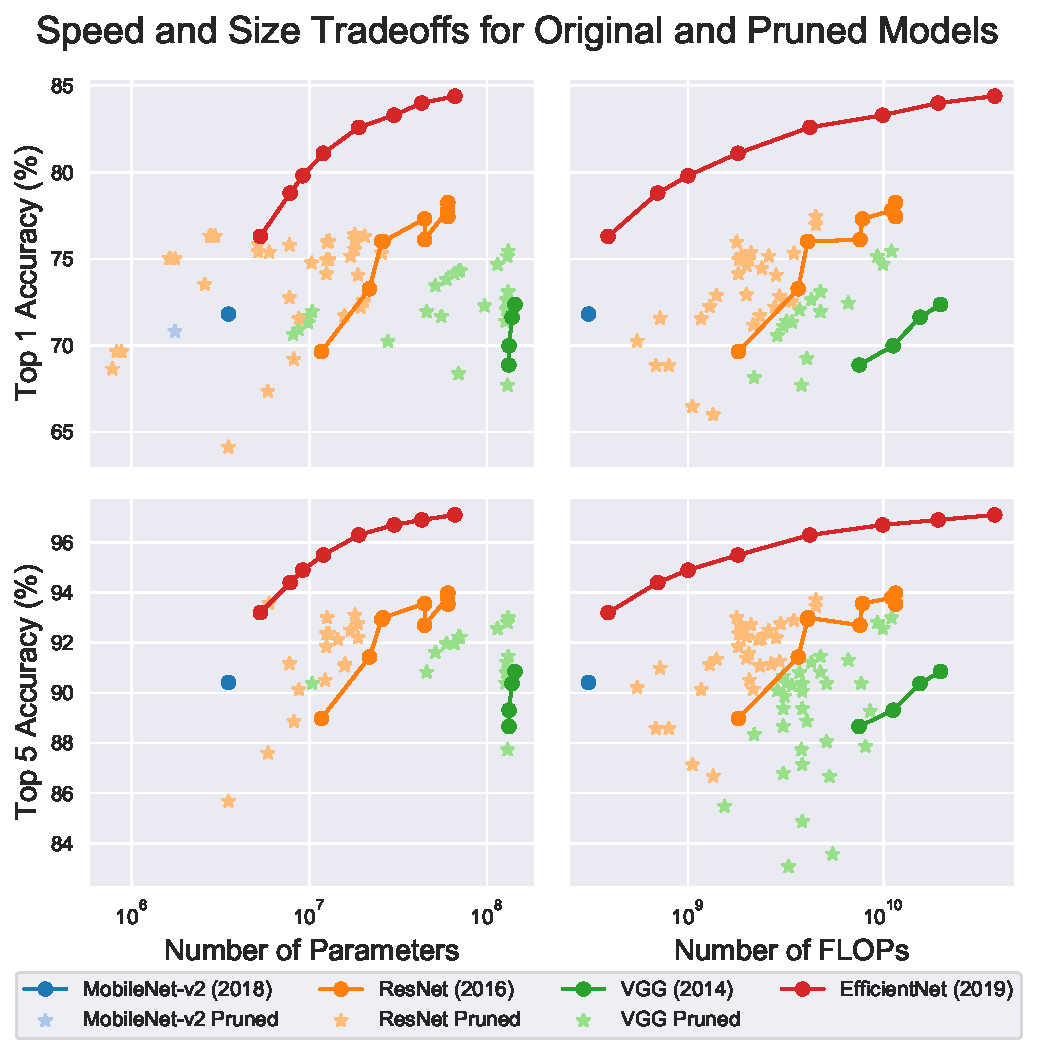
\includegraphics[width=\linewidth]{arch_vs_prune}
\vspace{-3mm}
\caption{Size and speed vs accuracy tradeoffs for different pruning methods and families of architectures. Pruned models sometimes outperform the original architecture, but rarely outperform a better architecture.}
\label{fig:arch_vs_prune}
\end{center}
\end{figure}
\vspace{3mm}

% ------------------------
% \subsubsection{Ignoring Recent Methods}
% \vspace{-3em}
\paragraph{Ignoring Recent Methods}
% ------------------------

% Even under the strong assumption that all pre-2010 methods are inferior, t
Even when considering only post-2010 approaches, there are still virtually no methods that have been shown to outperform all existing ``state-of-the-art'' methods. This follows from the fact, depicted in the top plot of Figure~\ref{fig:paper_comparisons_hist}, that there are dozens of modern papers---including many affirmed through peer review---that have never been compared to by any later study.
% We define a comparison here as reporting any numeric result for one's own method alongside any numeric result for the same (dataset, model) pair from the method in question. As we will discuss later in the section, this is a lax standard that does not necessarily imply that one method has meaningfully outperformed the other.
% Any of the associated authors could claim to have the best pruning method, since no one has ever even attempted to demonstrate otherwise.
% As emphasized previously, we believe that the main reason for this lack of comparison is not sloppiness or ill intent, but the reality that comparing to any given method is difficult or even impossible.

A related problem is that papers tend to compare to few existing methods. In the lower plot of Figure~\ref{fig:paper_comparisons_hist}, we see that more than a fourth of our corpus does not compare to any previously proposed pruning method, and another fourth compares to only one. Nearly all papers compare to three or fewer. This might be adequate if there were a clear progression of methods with one or two ``best'' methods at any given time, but this is not the case. % These observations hold for both published and unpublished papers.
% An additional and enabling factor appears to be lax community standards. In the lower plot of Figure~\ref{fig:paper_comparisons_hist}, we see that more than a fourth of our corpus \textit{does not compare to any existing pruning method}, and another fourth compares to only one. Nearly all papers compare to three or fewer. This might be adequate if there were a clear progression of methods with one or two ``best'' methods at any given time, but as this section argues, this is not the case. These facts hold for both published and unpublished papers.

% Even among modern papers, however, there are dozens of papers that can claim to be state-of-the-art, as measured by the absence

% Unfortunately, even if there were no methodological issues whatsoever with any of their experimental comparisons, this usually cannot have been the case even at the time the papers were written.

% In Figure~\ref{fig:paper_comparisons_hist}, we plot histograms of the number of papers comparing to a given method (top) and number of other papers that a given new paper compares to (bottom). The far left bar on the upper plot shows that there are over 30 papers that \textit{have never been compared to by anyone}, at least among all the papers we were able to find. In other words, there are at least 30 papers that can claim to be ``state-of-the-art''.

% In the lower plot, we see that the review standards for being ``state-of-the-art'' are remarkably lax.

\begin{figure}[h]
\begin{center}
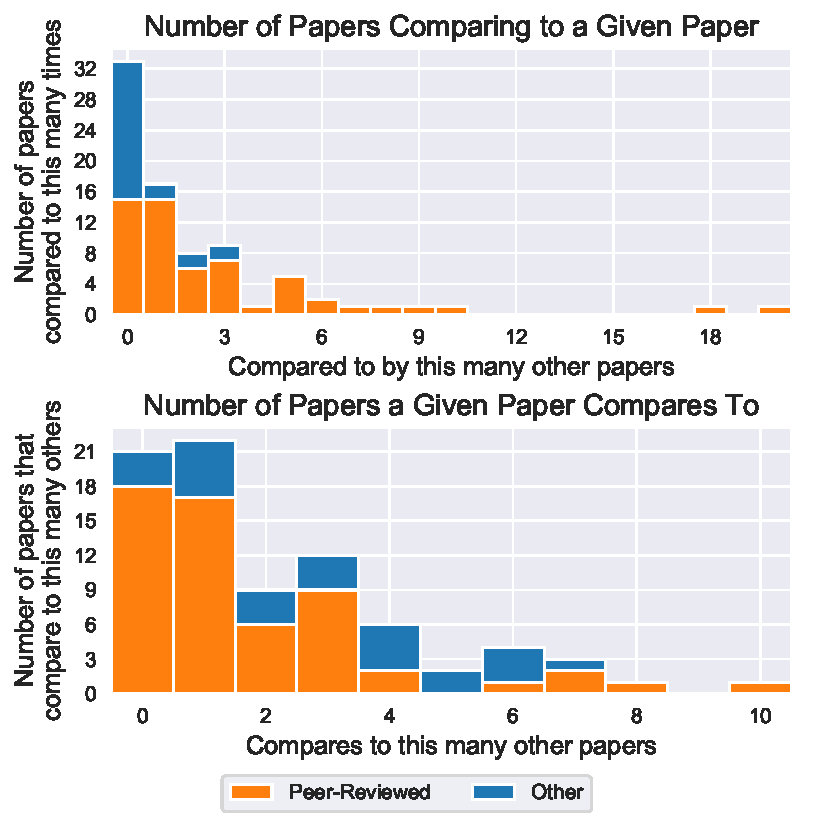
\includegraphics[width=\linewidth]{paper_comparisons_hist}
\caption{Reported comparisons between papers.
% \textit{Top)} More than a third of the papers in our corpus have no other paper purporting to outperform them. \textit{Bottom)} Most papers compare to at most one other paper, and often none. Peer-reviewed papers are less likely to be ignored, but do not make more comparisons to existing methods. % These patterns hold regardless of whether a paper is peer-reviewed.}
}
\label{fig:paper_comparisons_hist}
\end{center}
\end{figure}

% ------------------------------------------------
\subsection{Dataset and Architecture Fragmentation}
% ------------------------------------------------

% It appears that a major underlying cause for the absence of meaningful comparisons is the lack of standard datasets, architectures, and metrics. % This means that comparing to a given existing paper usually necessitates additional code to match the experimental setting of the particular paper in question, assuming the setting is reproducible enough to be matched at all. A few exemplary authors work hard to match many earlier experiments (e.g., \cite{dai-info-bottleneck, rethinking-net-pruning}), but, understandably, most avoid this as much as possible. % This causes new papers to introduce new experimental setups, creating a vicious cycle.
% This results in a self-perpetuating cycle of
% In this section, we describe the extent of the fragmentation in datasets and architectures. % We believe that this extreme fragmentation suggests a desparate need for standard benchmarks. % and by implication the desparate need for some form of standardization.

% The second core problem, which contributes to the first, is that there is no standard set of datasets and models that everyone uses. This
% results in 1) most comparisons involving at most one or two (dataset, architecture) combinations, 2) no ability to compare to other papers ``for free''---

% . This is far too little to establish that one method is superior to another, except perhaps in the case of perfectly representative tasks and large, consistent differences.

% As a first indication of how fragmented the reported results are, consider that

Among \npapers papers, we found results using 49 datasets, 132 architectures, and 195 (dataset, architecture) combinations. As shown in Table~\ref{tbl:common_combos}, even the most common combination of dataset and architecture---VGG-16 on ImageNet\footnote{We adopt the common practice of referring to the ILSVRC2012 training and validation sets as ``ImageNet.''} \cite{imagenet}---is used in only 22 out of \npapers papers. Moreover, three of the top six most common combinations involve MNIST \cite{mnist}. As \citet{google-state-of-sparsity} and others have argued, using larger datasets and models is essential when assessing how well a method works for real-world networks. MNIST results may be particularly unlikely to generalize, since this dataset differs significantly from other popular datasets for image classification. In particular, its images are grayscale, composed mostly of zeros, and possible to classify with over 99\% accuracy using simple models \cite{mnist-page}.

% since this dataset has several unusual properties. First, unlike other popular datasets for vision classification tasks, MNIST is not composed of natural images, but instead grayscale images that are mostly zeros. Second, the variance of image patterns across samples is smaller than other natural image datasets. Finally, even simple classifiers can obtain over 99\% test accuracy \cite{mnist-page} on MNIST.

% These properties mean that methods that work on MNIST may not work on larger-scale problems.

% TODO maybe switch to (dataset, model, efficiency metric, quality metric) ?

% \begin{table}[h!]
% \begin{centering}
% \begin{tabular}{ll|c}
% \multicolumn{2}{c}{(Dataset, Architecture) Pair} & \shortstack{Number of Papers \\ using Pair} \\
% % \vspace*{2pt}
% \toprule
% ImageNet & VGG-16 & 22 \\
% ImageNet & ResNet-50 & 15 \\
% MNIST & LeNet-5-Caffe & 14 \\
% CIFAR-10 & ResNet-56 & 14 \\
% MNIST & LeNet-300-100 & 12 \\
% MNIST & LeNet-5 & 11 \\
% ImageNet & CaffeNet & 10 \\
% CIFAR-10 & CIFAR-VGG (Torch) & 8 \\
% ImageNet & AlexNet & 8 \\
% ImageNet & ResNet-18 & 6 \\
% ImageNet & ResNet-34 & 6 \\
% CIFAR-10 & ResNet-110 & 5 \\
% CIFAR-10 & PreResNet-164 & 4 \\
% CIFAR-10 & ResNet-32 & 4 \\
% % \bottomrule
% % ImageNet, ResNet-101 & 3 \\
% % ImageNet, GoogLeNet & 3 \\
% % CIFAR-100, PreResNet-164 & 3 \\
% % CIFAR-10, VGG-19 & 3 \\
% % CIFAR-10, ResNet-20 & 3 \\
% % CIFAR-10, VGG-netslim & 3 \\
% % CIFAR-10, ResNet-18 & 3 \\
% % CUB200-2011, VGG-16 & 3 \\
% % CIFAR-100, VGG-Torch-CIFAR10 & 3 \\
% % CIFAR-10, DenseNet-40 & 3 \\
% % CIFAR-100, VGG-19 & 2 \\
% % CIFAR-10, Cifar-net & 2 \\
% % CamVid, SegNet & 2 \\
% % CIFAR-10, WRN-28-10 & 2 \\
% % CIFAR-10, WRN-22-8 & 2 \\
% % CIFAR-100, DenseNet-40 & 2 \\
% % ImageNet, VGG-Tiny & 2 \\
% % ImageNet, VGG-GAP & 2 \\
% % ImageNet, VGG-A+BN-noDrop & 2 \\
% % MNIST, fc300-1000-300 & 2 \\
% % MNIST, fc500-300-100 & 2 \\
% % ImageNet, SqueezeNet & 2 \\
% % CIFAR-10, PreResNet-110 & 2 \\
% % CIFAR-100, WRN-28-10 & 2 \\
% % ImageNet, MobileNet & 2 \\
% % Pascal VOC 2007, VGG-16 & 2 \\
% % CIFAR-10, Plain-20 & 2 \\
% % CIFAR-100, WRN-16-4 & 2 \\
% % CIFAR-10, ResNet-50 & 2 \\
% \end{tabular}
% \end{centering}
% \caption{All combinations of dataset and architecture used in at least 4 out of \npapers papers.
% % To have a clear state-of-the-art, there should be numerous combinations used by a large fraction of papers.
% }
% \label{tbl:common_combos}
% \vspace*{1mm}
% \end{table}

% ------------------------------------------------
\subsection{Metrics Fragmentation}
% ------------------------------------------------

\begin{table}[t]
\begin{centering}
\begin{tabular}{ll|c}
\multicolumn{2}{c}{(Dataset, Architecture) Pair} & \shortstack{Number of Papers \\ using Pair} \\
% \vspace*{2pt}
\toprule
ImageNet & VGG-16 & 22 \\
ImageNet & ResNet-50 & 15 \\
MNIST & LeNet-5-Caffe & 14 \\
CIFAR-10 & ResNet-56 & 14 \\
MNIST & LeNet-300-100 & 12 \\
MNIST & LeNet-5 & 11 \\
ImageNet & CaffeNet & 10 \\
CIFAR-10 & CIFAR-VGG (Torch) & 8 \\
ImageNet & AlexNet & 8 \\
ImageNet & ResNet-18 & 6 \\
ImageNet & ResNet-34 & 6 \\
CIFAR-10 & ResNet-110 & 5 \\
CIFAR-10 & PreResNet-164 & 4 \\
CIFAR-10 & ResNet-32 & 4 \\
% \bottomrule
% ImageNet, ResNet-101 & 3 \\
% ImageNet, GoogLeNet & 3 \\
% CIFAR-100, PreResNet-164 & 3 \\
% CIFAR-10, VGG-19 & 3 \\
% CIFAR-10, ResNet-20 & 3 \\
% CIFAR-10, VGG-netslim & 3 \\
% CIFAR-10, ResNet-18 & 3 \\
% CUB200-2011, VGG-16 & 3 \\
% CIFAR-100, VGG-Torch-CIFAR10 & 3 \\
% CIFAR-10, DenseNet-40 & 3 \\
% CIFAR-100, VGG-19 & 2 \\
% CIFAR-10, Cifar-net & 2 \\
% CamVid, SegNet & 2 \\
% CIFAR-10, WRN-28-10 & 2 \\
% CIFAR-10, WRN-22-8 & 2 \\
% CIFAR-100, DenseNet-40 & 2 \\
% ImageNet, VGG-Tiny & 2 \\
% ImageNet, VGG-GAP & 2 \\
% ImageNet, VGG-A+BN-noDrop & 2 \\
% MNIST, fc300-1000-300 & 2 \\
% MNIST, fc500-300-100 & 2 \\
% ImageNet, SqueezeNet & 2 \\
% CIFAR-10, PreResNet-110 & 2 \\
% CIFAR-100, WRN-28-10 & 2 \\
% ImageNet, MobileNet & 2 \\
% Pascal VOC 2007, VGG-16 & 2 \\
% CIFAR-10, Plain-20 & 2 \\
% CIFAR-100, WRN-16-4 & 2 \\
% CIFAR-10, ResNet-50 & 2 \\
\end{tabular}
\end{centering}
\caption{All combinations of dataset and architecture used in at least 4 out of \npapers papers.
% To have a clear state-of-the-art, there should be numerous combinations used by a large fraction of papers.
}
\label{tbl:common_combos}
\vspace*{1mm}
\end{table}

As depicted in Figure~\ref{fig:prune_grid}, papers report a wide variety of metrics and operating points, making it difficult to compare results. Each column in this figure is one (dataset, architecture) combination taken from the four most common combinations\footnote{We combined the results for AlexNet and CaffeNet, which is a slightly modified version of AlexNet \cite{caffenet}, since many authors refer to the latter as ``AlexNet,'' and it is often unclear which model was used.}, excluding results on MNIST. Each row is one pair of metrics. Each curve is the efficiency vs accuracy tradeoff obtained by one method.\footnote{Since what counts as one method can be unclear, we consider all results from one paper to be one method except when two or more named methods within the paper report using at least one identical x-coordinate (i.e., when the paper's results can't be plotted as one curve).} Methods are color-coded by year.

It is hard to identify any consistent trends in these plots, aside from the existence of a tradeoff between efficiency and accuracy. A given method is only present in a small subset of plots. Methods from later years do not consistently outperform methods from earlier years. Methods within a plot are often incomparable because they report results at different points on the x-axis. Even when methods are nearby on the x-axis, it is not clear whether one meaningfully outperforms another since neither reports a standard deviation or other measure of central tendency. Finally, most papers in our corpus do not report any results with any of these common configurations.

\begin{figure*}[hbt!]
\begin{center}
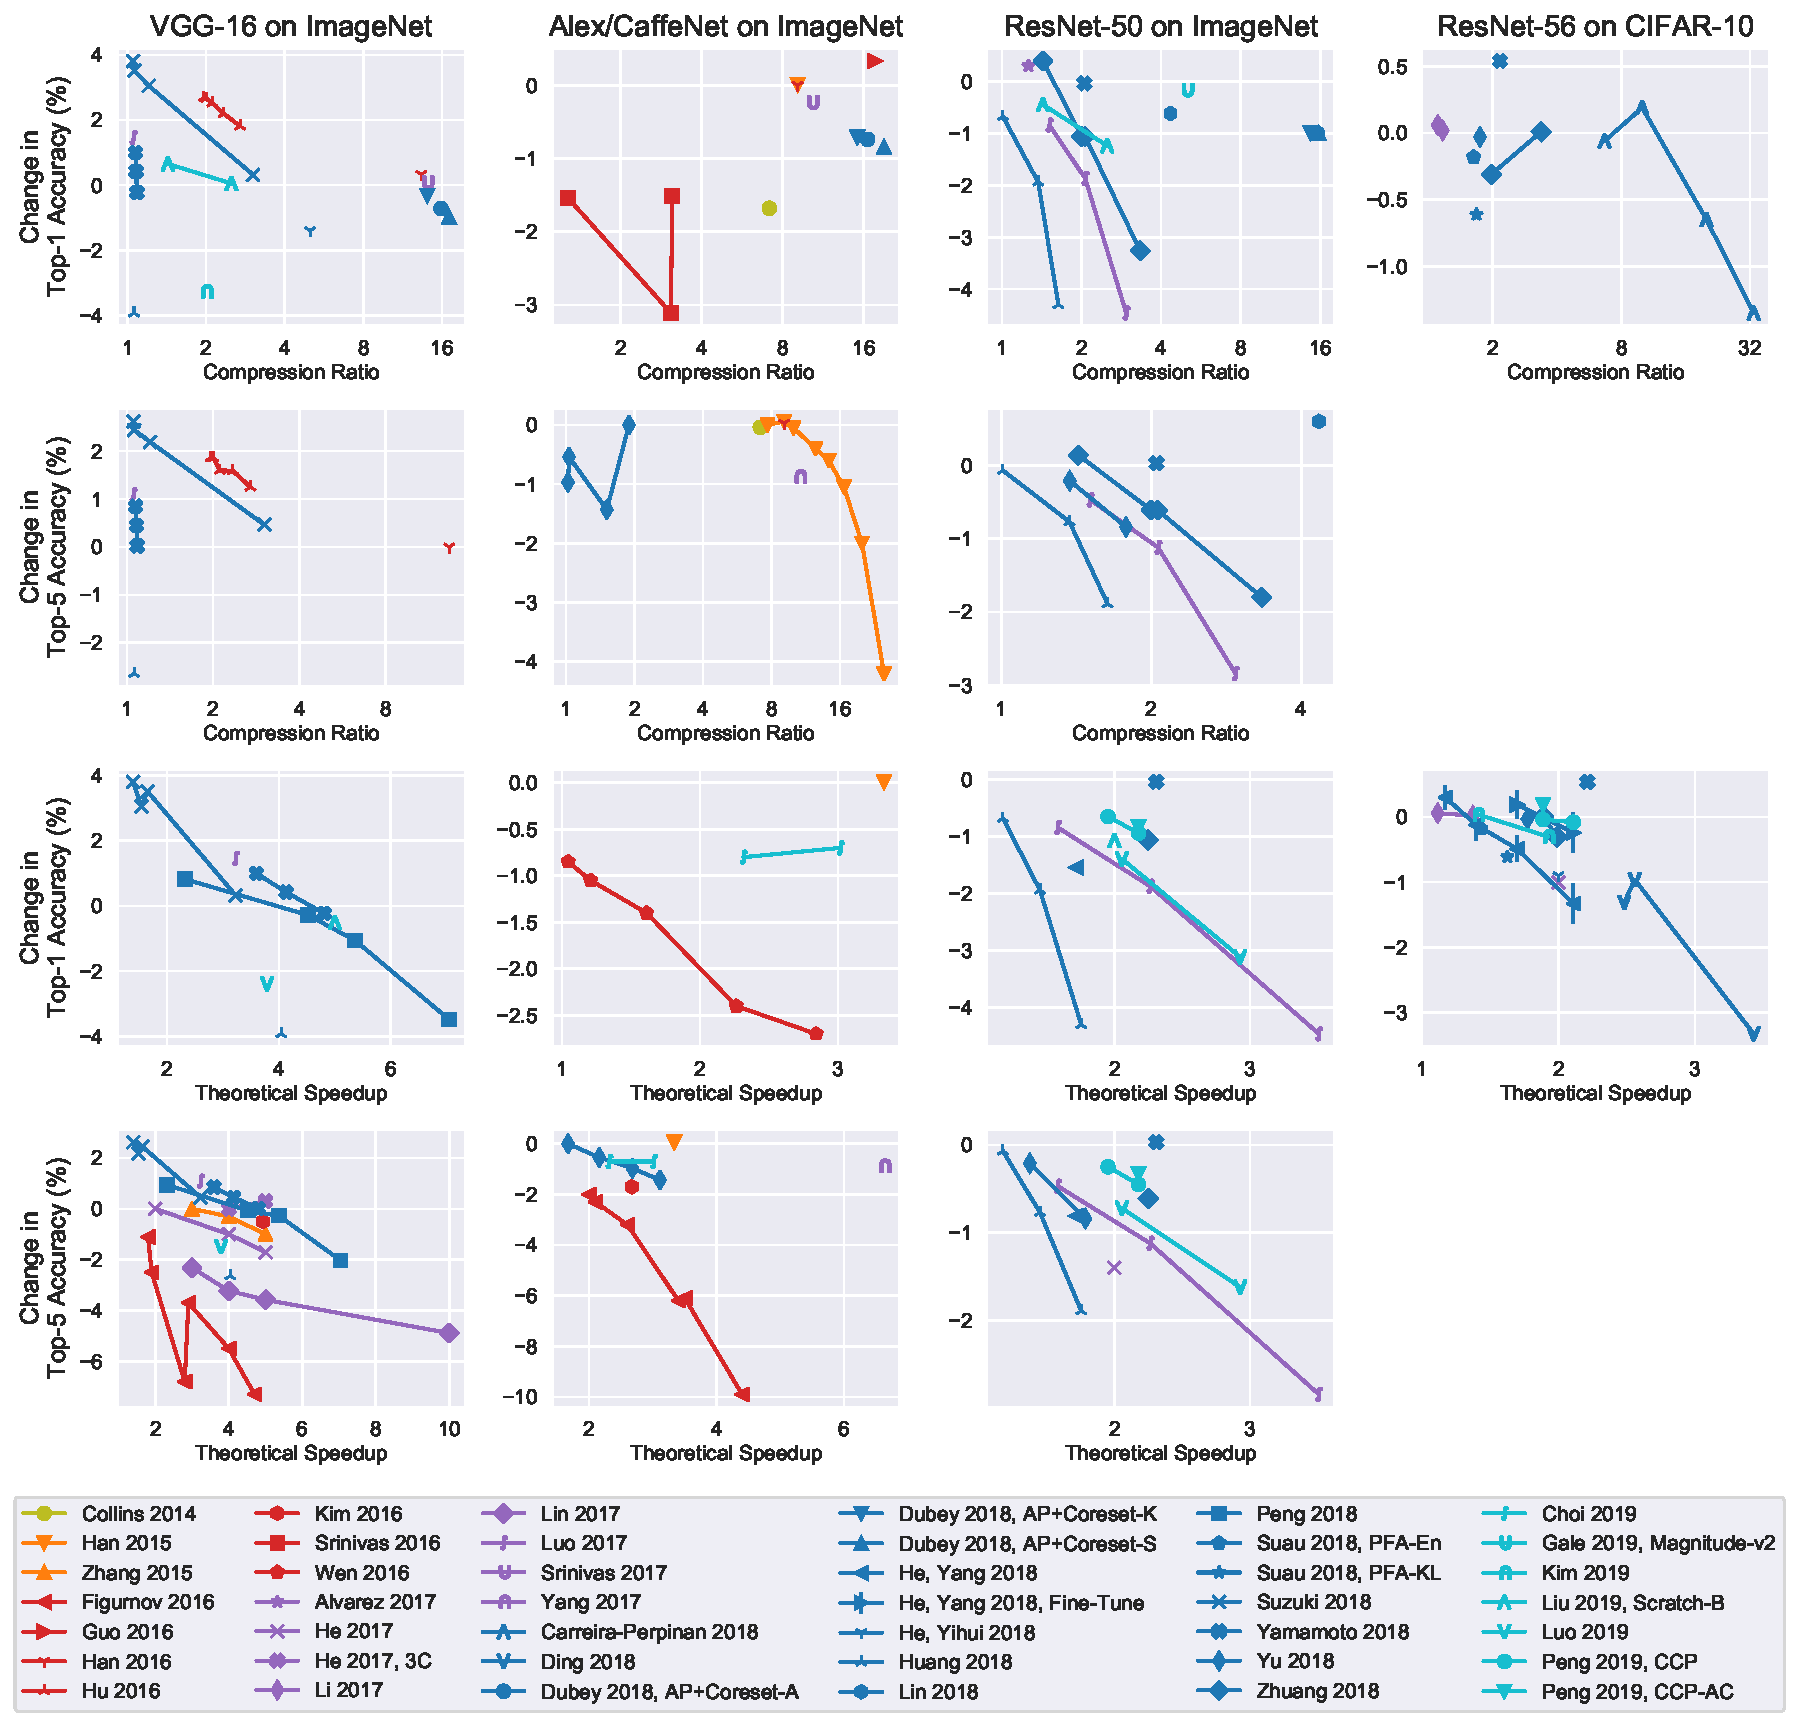
\includegraphics[width=\linewidth]{all_pruning_curves}
\caption{Fragmentation of results. Shown are all self-reported results on the most common (dataset, architecture) combinations. Each column is one combination, each row shares an accuracy metric (y-axis), and pairs of rows share a compression metric (x-axis). Up and to the right is always better. Standard deviations are shown for He 2018 on CIFAR-10, which is the only result that provides any measure of central tendency.
% Observe that each combination of dataset, architecture, and metrics (one subplot) has results from only a small fraction of the papers. Even when these factors agree, different papers often obtain incomparable results since they are better in one respect but worse in another. Methods are color-coded by year, and there appears to be no clear progress over time. Later methods are sometimes strictly worse than earlier ones.
As suggested by the legend, only 37 out of the \npapers papers in our corpus report any results using any of these configurations.}
\label{fig:prune_grid}
\end{center}
\vspace{-4mm}
\end{figure*}

% ------------------------------------------------
% \subsection{Incomplete Characterization of Results}
\subsection{Incomplete Characterization of Results}
% ------------------------------------------------

% As shown in Figure~\ref{fig:prune_grid}, many methods are not comparable because they use different combinations of models, datasets, and metrics, as well as disparate efficiency levels in their efficiency vs accuracy tradeoff curves.
% Recall that a pruning method must balance both efficiency and accuracy, and that this tradeoff can be characterized in terms of a curve of (efficiency, accuracy) pairs associated with a given dataset and model. As we discussed previously, methods with non-overlapping ranges of their reported curves, or with different datasets and models, cannot be directly compared.

If all papers reported a wide range of points in their tradeoff curves across a large set of models and datasets, there might be some number of direct comparisons possible between any given pair of methods. %, even if the overall sets of reported results differed.
% One factor exacerbating this is that authors report few (dataset, architecture) pairs as well as few measurements to characterize each pair's tradeoff curve.
As we see in the upper half of Figure~\ref{fig:numresults_stats}, however, most papers use at most three (dataset, architecture) pairs; and as we see in the lower half, they use at most three---and often just one---point to characterize each curve. Combined with the fragmentation in experimental choices, this means that different methods' results are rarely directly comparable. Note that the lower half restricts results to the four most common (dataset, architecture) pairs.

\begin{figure}[h]
\begin{center}
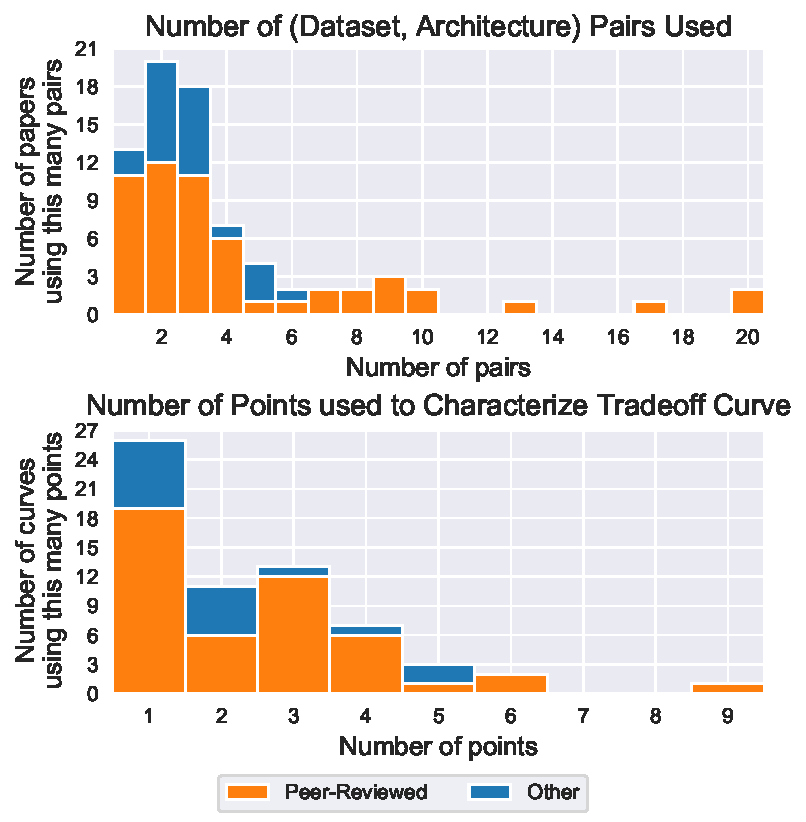
\includegraphics[width=\linewidth]{numresults_stats}
\caption{Number of results reported by each paper, excluding MNIST. \textit{Top)} Most papers report on three or fewer (dataset, architecture) pairs. \textit{Bottom)} For each pair used, most papers characterize their tradeoff between amount of pruning and accuracy using a single point in the efficiency vs accuracy curve. In both plots, the pattern holds even for peer-reviewed papers.}
\label{fig:numresults_stats}
\end{center}
\end{figure}

% ------------------------------------------------
\subsection{Confounding Variables} \label{sec:confounding}
% ------------------------------------------------
% Suppose that Paper A compares to Paper B using a large number of the same architectures on the same datasets, reports the same metrics, evaluates their method at numerous operating points, which are themselves identical to those used in Paper B, and obtains better results than those reported in Paper B at all operating points. Can we conclude that Paper A's method outperforms Paper B's?
% Unfortunately, we may not be able to. The problem is that using reported results fails to account for numerous confounding variables. Some variables of particular interest include:

% % ------------------------
% \subsubsection{Common Confounders}
% % ------------------------
Even when comparisons include the same datasets, models, metrics, and operating points, other confounding variables still make meaningful comparisons difficult. Some variables of particular interest include:
\begin{itemize}[leftmargin=4mm]
    % \itemsep-1.5pt
    \itemsep2pt
    \vspace{-3.5mm}
    % \item Initial trained parameters. Initially worse models might be easier or harder to improve.
    \item Accuracy and efficiency of the initial model
    \item Data augmentation and preprocessing
    \item Random variations in initialization, training, and fine-tuning. This includes choice of optimizer, hyperparameters, and learning rate schedule.
    \item Pruning and fine-tuning schedule
    % (how often to prune throughout fine-tuning, how much pruning at a time, total fine-tuning epochs, etc).
    % \item Fine-tuning settings, such as number of epochs of fine-tuning.
    \item Deep learning library. Different libraries are known to yield different accuracies for the same architecture and dataset \cite{unreproducibleCurtis, unreproducible3} and may have subtly different behaviors \cite{kerasBnWeird}.
    \item Subtle differences in code and environment that may not be easily attributable to any of the above variations \cite{unreproducible0, unreproducible1, unreproducible4}.
\end{itemize}
% \vspace{-10pt}

In general, it is not clear that any paper can succeed in accounting for all of these confounders unless that paper has both used the same code as the methods to which it compares and reports enough measurements to average out random variations. This is exceptionally rare, with \citet{google-state-of-sparsity} and \citet{rethinking-net-pruning} being arguably the only examples. Moreover, neither of these papers introduce novel pruning methods \textit{per se} but are instead inquiries into the efficacy of existing methods.

% ------------------------
% \subsubsection{Common Mitigation Practices can be Inadequate}
% \paragraph{Common Mitigation Practices can be Inadequate}
% ------------------------

Many papers attempt to account for subsets of these confounding variables. A near universal practice in this regard is reporting change in accuracy relative to the original model, in addition to or instead of raw accuracy. This helps to control for the accuracy of the initial model. However, as we demonstrate in Section~\ref{sec:bench}, this is not sufficient to remove initial model as a confounder. Certain initial models can be pruned more or less efficiently, in terms of the accuracy vs compression tradeoff. This holds true even with identical pruning methods and all other variables held constant.

% we did not find any empirical or theoretical evidence that examining only changes is sufficient to remove initial model accuracy as a confounder. I.e., it could be the case that initially worse models are easier (or harder) to prune without accuracy degradation.

%The thinking is that a method that reduces accuracy from 92\% to 91\% should be considered worse than a method that increases it from 88\% to 90\%, even though the latter obtains a lower final accuracy. This is probably correct, but we did not find any empirical or theoretical evidence that examining only changes is sufficient to remove initial model accuracy as a confounder. I.e., it could be the case that initially worse models are easier (or harder) to prune without accuracy degradation.
% It could be the case that a worse model is likely easier to ``improve'' by pruning, if only because fine-tuning affords one a chance to get less unlucky than whomever initially trained the model (and possibly to apply more recent training methods).

% ------------------------
% \subsubsection{Impact of Fine-Tuning}
% \subsubsection{Impact of Confounders}
% \paragraph{Impact of Confounders}
% ------------------------

% One might wonder whether the impact of these confounders is actually significant relative to that of pruning method choice. % After all, random variations typically perturb accuracies for a given pruned model on ImageNet by less than half a percentage point [], and the relative efficacy of ImageNet image classifiers appears to hold even for novel large-scale datasets [].
\vspace{2mm}
There are at least two more empirical reasons to believe that confounding variables can have a significant impact. First, as one can observe in Figure~\ref{fig:prune_grid}, methods often introduce changes in accuracy of much less than 1\% at reported operating points. This means that, even if confounders have only a tiny impact on accuracy, they can still have a large impact on which method appears better. % This is particularly true in the absence of any sort of error bars.

\vspace{2mm}
Second, as shown in Figure~\ref{fig:magnitude_vs_nonmagnitude}, existing results demonstrate that different training and fine-tuning settings can yield nearly as much variability as different methods. Specifically, consider 1) the variability introduced by different fine-tuning methods for unstructured magnitude-based pruning (Figure 6 top) and 2) the variability introduced by entirely different pruning methods (Figure 6 bottom). The variability between fine-tuning methods is nearly as large as the variability between pruning methods.
%Specifically, consider two sets of tradeoff curves: 1) those for a single method (iterative, unstructured, magnitude-based pruning) using different implementations and fine-tuning practices, and 2) those for all other methods. If method made far more difference than training and fine-tuning, then the former set of curves should exhibit far less variation than the latter. As Figure~\ref{fig:magnitude_vs_nonmagnitude} depicts however, this is not the case---the within-method variation is nearly as large as the between-method variation.
 % As we see in , these two sets of curves appear to vary in quality as much as the tradeoff curves for different methods.
\begin{figure}[h]
\begin{center}
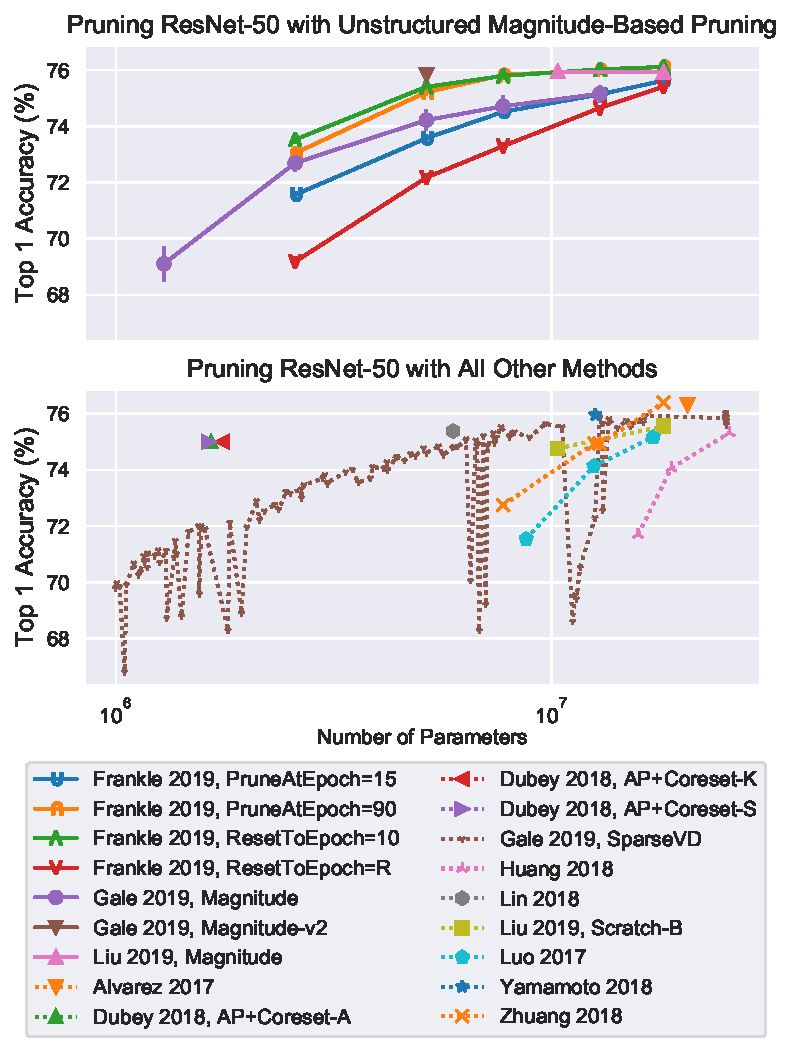
\includegraphics[width=\linewidth]{magnitude_vs_nonmagnitude}
\caption{Pruning ResNet-50 on ImageNet. Methods in the upper plot all prune weights with the smallest magnitudes, but differ in implementation, pruning schedule, and fine-tuning. The variation caused by these variables is similar to the variation across different pruning methods, whose results are shown in the lower plot. All results are taken from the original papers.}
\label{fig:magnitude_vs_nonmagnitude}
\end{center}
\vspace*{3mm}
\end{figure}
